\documentclass[12pt, twoside]{article}
\usepackage[letterpaper, margin=1in, headsep=0.5in]{geometry}
\usepackage[english]{babel}
\usepackage[utf8]{inputenc}
\usepackage{amsmath}
\usepackage{amsfonts}
\usepackage{amssymb}
\usepackage{tikz}
%\usetikzlibrary{quotes, angles}

\usepackage{graphicx}
\usepackage{enumitem}
\usepackage{multicol}

\usepackage{fancyhdr}
\pagestyle{fancy}
\fancyhf{}
\renewcommand{\headrulewidth}{0pt} % disable the underline of the header

\fancyhead[LE]{\thepage}
\fancyhead[RO]{\thepage \\ Name: \hspace{4cm} \,\\}
\fancyhead[LO]{BECA / Dr. Huson / Geometry\\* Unit 7: Similarity\\* 3 January 2020}

\begin{document}
\subsubsection*{7.2 Homework: Similar triangles, dilations}
  \begin{enumerate}

  \item The diagram below shows $\triangle ABC$, with $\overline{AEB}$, $\overline{ADC}$, and $\angle ACB \cong \angle AED$. $AB=8$, $AD=4$, and $DE=2$.
    \begin{multicols}{2}
      \begin{enumerate}
      \item $\triangle ADE \rightarrow$ \rule{2cm}{0.15mm} \vspace{1cm}
      \item $\overline{AD} \rightarrow$ \rule{2cm}{0.15mm} \vspace{1cm}
      \item What is the scale factor?\\[0.5cm] $k=$  \rule{2cm}{0.15mm}
      \item What is the length of $\overline{BC}$?
    \end{enumerate}
      \begin{tikzpicture}[scale=1.3]
        \draw [thick]
        (0,0) node[above right] {$A$}--
        (230:6) node[below left] {$B$}--
        (260:4.75) node[below right] {$C$}--cycle;
        \draw [thick]
        (230:2.375) node[above left] {$E$}--
        (260:3) node[right] {$D$}--cycle;
      \end{tikzpicture}
    \end{multicols} \vspace{2cm}
    
  \item Given $\triangle ABC \sim \triangle ADE$ with sides $AC = 9$, $BC = 6$, $AB = 12$, and of $DE = 10$ find the scale factor $k$ and the lengths $AD$ and $AE$. Then find $CD$. \vspace{1cm}
  \begin{multicols}{2}
    \begin{enumerate}
      \item $k=$ \vspace{1cm}
      \item $AD=$ \vspace{1cm}
      \item $AE=$ \vspace{1cm}
      \item $CD=$
    \end{enumerate}
    \begin{flushright}
      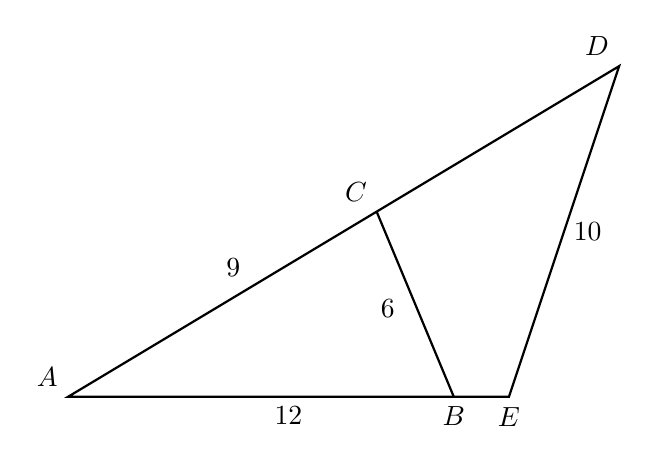
\begin{tikzpicture}[scale=0.7]
        \draw [-, thick] (0,0) node[above left]{$A$}--
        (8,0) node[below]{$E$}--
        (10,6) node[above left]{$D$}--cycle;
        \draw [thick] (7,0)--(5.6,3.36);
        \node at (7,0) [below]{$B$};
        \node at (5.6,3.36) [above left]{$C$};
        \node at (4, 0) [below]{$12$};
        \node at (3,2) [above]{$9$};
        \node at (9, 3) [right]{$10$};
        \node at (5.5, 1.6) [right]{$6$}; \vspace{1cm}
      \end{tikzpicture}
    \end{flushright} 
  \end{multicols}\vspace{1.5cm}

\newpage
  \item Given $\triangle ABP \sim \triangle JKP$ as shown below. $AB=9.6$, $AP=12.0$, $BP=6.3$, and $JP=18.0$. Find $KP$.
  \begin{flushright}
  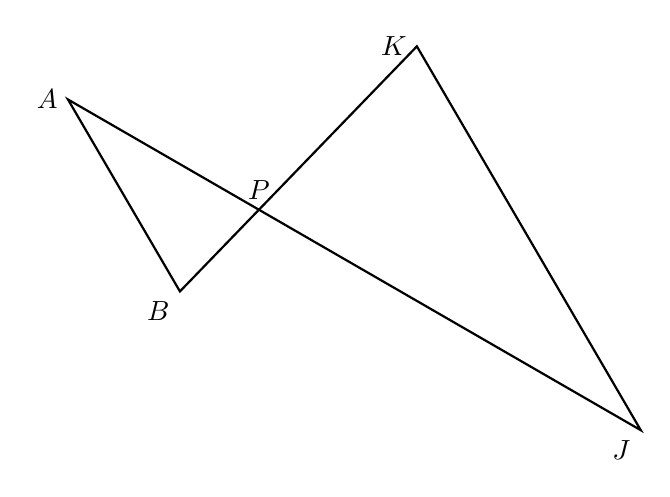
\begin{tikzpicture}[rotate=-30, scale=1.4]
      \draw [thick]
        (-0.25,-1)node[below left]{$B$}--
        (0.5,2)node[left]{$K$}--
        (4,0)node[below left]{$J$}--
        (0,0)node[above]{$P$}--
        (-2,0)node[left]{$A$}--cycle;
    \end{tikzpicture}
    \end{flushright}
    \vspace{2cm}

  \item In the diagram below, the chords $\overline{AE}$ and $\overline{BD}$ intersect at $C$. Given $\triangle ABC \sim \triangle DEC$, $AB=2$, $DE=4$, and $AC=3$. Determine the length of $\overline{CD}$.
      \begin{center}
      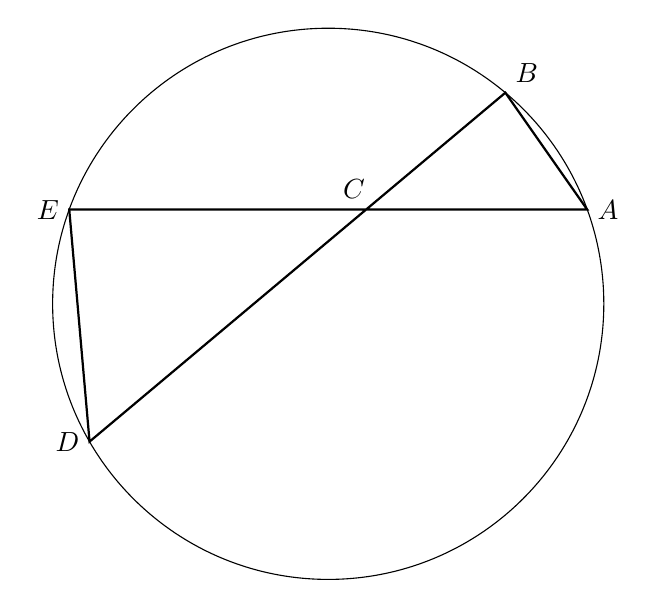
\begin{tikzpicture}[scale=.7]
        \draw (0,0) circle[radius=5];
        \draw [thick]
        (20:5) node[right] {$A$}--
        (160:5) node[left] {$E$}--
        (210:5) node[left] {$D$}--
        (50:5) node[above right] {$B$}--cycle;
        \draw (75:1.8) node[above] {$C$};
      \end{tikzpicture}
    \end{center}

\newpage
  \item In the diagram below of $\triangle ABC$, $D$ is a point on $\overline{BA}$, $E$ is a point on $\overline{BC}$, and $\overline{DE}$ is drawn. \\*[2pt] 
  If $BD=5$, $DA=12$, and $BE=7$, what is the length of $\overline{BC}$ so that $\overline{AC} \parallel \overline{DE}$?
  \begin{flushright}
      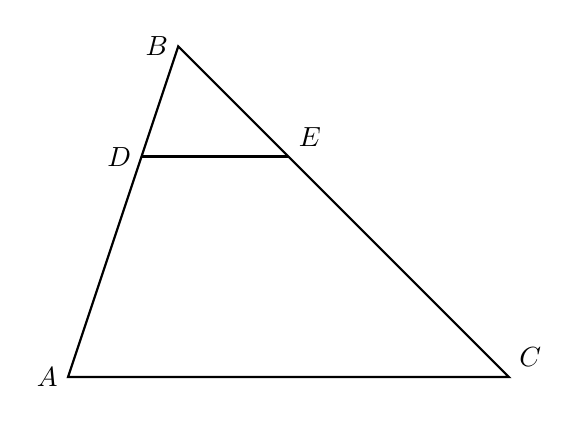
\begin{tikzpicture}[scale=0.7]
        \draw [thick]
        (0,0)node[left]{$A$}--
        (8,0)node[above right]{$C$}--
        (2,6)node[left]{$B$}--cycle;
        \draw [thick]
        (4/3,4)node[left]{$D$}--
        (4,4)node[above right]{$E$};
      \end{tikzpicture}
    \end{flushright} \vspace{1cm}
  
  \item Triangle $ADE$ and its midline $\overline{BC}$ are drawn, with $B$ the midpoint of $\overline{AD}$ and $C$ the midpoint of $\overline{AE}$. The two medians $\overline{BE}$ and $\overline{CD}$ are drawn, as shown, intersecting in point $F$, the centroid.\\[0.25cm]
  $\triangle FCB \sim \triangle FDE$ with scale factor $k=2$.\\[1cm]
  Given $BC=7$, find $DE$. \\[1cm] Given $BF=3$, find $FE$.
  \begin{flushright}
      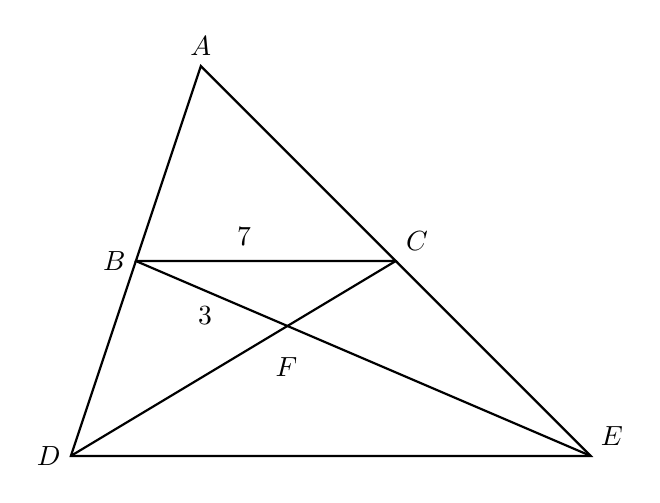
\begin{tikzpicture}[scale=0.55]
        \draw [thick]
        (0.5,1.5)node[left]{$B$}--
        (6.5,1.5)node[above right]{$C$}--
        (2,6)node[above]{$A$}--cycle;
        \draw [thick]
        (0.5,1.5)--
        (-1,-3)node[left]{$D$}--
        (11,-3)node[above right]{$E$}--(6.5,1.5);
        \draw [thick] (0.5,1.5)--(11,-3);
        \draw [thick] (6.5,1.5)--(-1,-3);
        \node at (3,2.5)[below]{$7$};
        \node at (3.5, -0.5)[below right]{$F$};
        \node at (2.1, -0.2)[above]{$3$};
        %\node at (-0.7, -1)[above]{$5$};
      \end{tikzpicture}
    \end{flushright} \vspace{1cm}
  
\newpage
  \item The side $\overline{AB}$ of triangle $ABC$ is extended and an altitude to the vertex $C$ is drawn, as shown below. The triangle's height is $h=8.1$ and its base measures $AB=13.4$. Find the area of the triangle.
    \begin{flushright}
      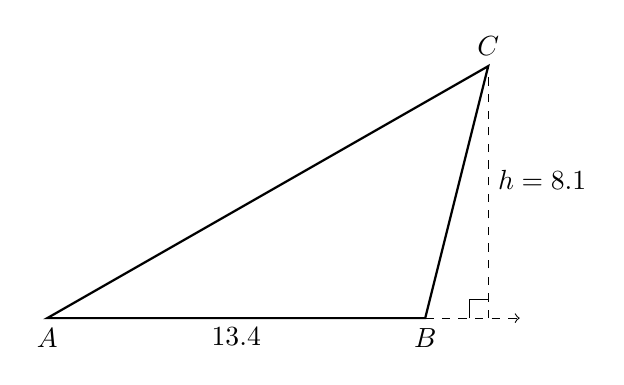
\begin{tikzpicture}[scale=0.8]
        \draw [thick]
          (0,0)node[below]{$A$}--
          (6,0)node[below]{$B$}--
          (7,4)node[above]{$C$} --cycle;
      \draw [dashed] (7,0)--(7,4);
      \draw [dashed, ->] (6,0)--(7.5,0);
      \draw (7,0)++(-0.3,0)--++(0,0.3)--+(0.3,0);
      \node at (7,2.2)[right]{$h=8.1$};
      \node at (3,0)[below]{$13.4$};
      \end{tikzpicture}
    \end{flushright}
    
  \item Given $\triangle DEF$ with height $h=10$ and base measuring $DE=12$. 
    \begin{enumerate}
    \item Find the area of $\triangle DEF$.
      \begin{flushright}
        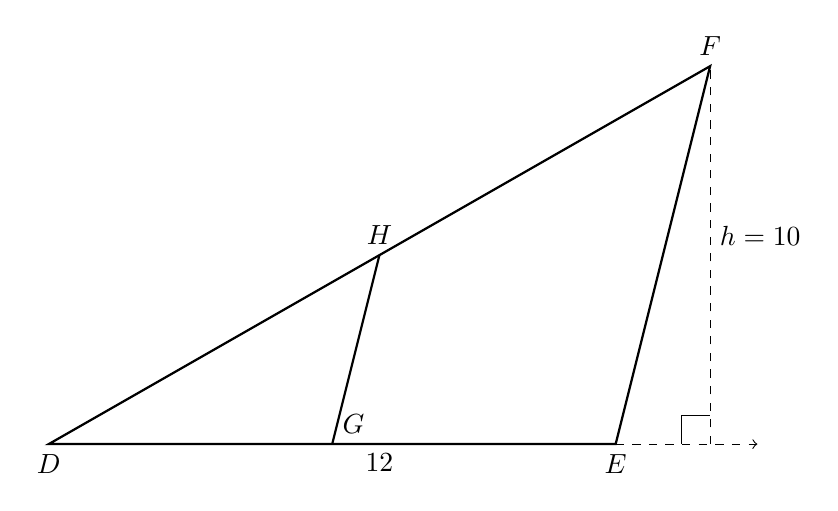
\begin{tikzpicture}[scale=1.2]
          \draw [thick]
            (0,0)node[below]{$D$}--
            (6,0)node[below]{$E$}--
            (7,4)node[above]{$F$} --cycle;
            \draw [thick]
            (3.5,2)node[above]{$H$}--
            (3,0)node[above right]{$G$};
        \draw [dashed] (7,0)--(7,4);
        \draw [dashed, ->] (6,0)--(7.5,0);
        \draw (7,0)++(-0.3,0)--++(0,0.3)--+(0.3,0);
        \node at (7,2.2)[right]{$h=10$};
        \node at (3.5,0)[below]{$12$};
        \end{tikzpicture}
      \end{flushright}
      \item A dilation centered at $D$ with $k=0.5$ maps $\triangle DEF \rightarrow \triangle DGH$. Find the base and height of $\triangle DGH$ and its area.
      
\end{enumerate}


\end{enumerate}
\end{document}